\section{Experimental Results} \label{apx:results}
Here we include the full breakdown of all experimental results. Tables \ref{tab:eigenworms_all} and \ref{tab:bidmc_all} include all results from the EigenWorms and BIDMC datasets respectively. We also give the heatmap style breakdown of the BIDMC results analogous to figure \ref{fig:eigenworms} in figure \ref{fig:bidmc_heatmap}.

\begin{table}[t]
    \begin{center}
        \begin{tabular}{ccccc}
        \toprule
        \textbf{Model} & \textbf{Step} & \textbf{Test Accuracy} & \textbf{Time (Hrs)} & \textbf{Memory (Mb)} \\
        \midrule
        & 1    &  62.4 $\pm$ 12.1 &          22.0 &         176.5 \\
          & 2    &   69.2 $\pm$ 4.4 &          14.6 &          90.6 \\
          & 4    &  66.7 $\pm$ 11.8 &           5.5 &          46.6 \\
          & 8    &  64.1 $\pm$ 13.3 &           3.1 &          24.3 \\
        \multirow{2}{*}{NCDE$_1$}  & 16   &  64.1 $\pm$ 16.8 &           1.5 &          13.4 \\
         & 32   &  64.1 $\pm$ 14.3 &           0.5 &           8.0 \\
          & 64   &   56.4 $\pm$ 6.8 &           0.4 &           5.2 \\
          & 128  &   48.7 $\pm$ 2.6 &           0.1 &           3.9 \\
          & 256  &   42.7 $\pm$ 3.0 &           0.1 &           3.2 \\
          & 512  &   44.4 $\pm$ 5.3 &           0.0 &           2.9 \\
        \midrule
          & 2    &  \textbf{76.1 $\pm$ 13.2} &           9.8 &         354.3 \\
          & 4    &   \textbf{83.8 $\pm$ 3.0} &           2.4 &         180.0 \\
          & 8    &   \textbf{77.8 $\pm$ 5.9} &           2.1 &          94.2 \\
          & 16   &   \textbf{78.6 $\pm$ 3.9} &           1.3 &          50.2 \\
        NCDE$_2$  & 32   &  67.5 $\pm$ 12.1 &           0.7 &          28.1 \\
          & 64   &   73.5 $\pm$ 7.8 &           0.4 &          17.2 \\
          & 128  &   \textbf{76.1 $\pm$ 5.9} &           0.2 &           7.8 \\
          & 256  &  \textbf{72.6 $\pm$ 12.1} &           0.1 &           8.9 \\
          & 512  &  \textbf{69.2 $\pm$ 11.8} &           0.0 &           7.6 \\
        \hdashline\noalign{\vskip 0.5ex}
          & 2    &   66.7 $\pm$ 4.4 &           7.4 &        1766.2 \\
          & 4    &   76.9 $\pm$ 9.2 &           2.8 &         856.8 \\
          & 8    &   70.1 $\pm$ 6.5 &           1.3 &         460.7 \\
          & 16   &   73.5 $\pm$ 3.0 &           1.4 &         243.7 \\
        NCDE$_3$  & 32   &   \textbf{75.2 $\pm$ 3.0} &           0.6 &         134.7 \\
          & 64   &  \textbf{74.4 $\pm$ 11.8} &           0.3 &          81.0 \\
          & 128  &   68.4 $\pm$ 8.2 &           0.1 &          53.3 \\
          & 256  &   60.7 $\pm$ 8.2 &           0.1 &          40.2 \\
          & 512  &  62.4 $\pm$ 10.4 &           0.0 &          33.1 \\
        \bottomrule
        \end{tabular}
    \end{center}
    \caption{Test set accuracy (in \%), memory usage and training time on the UEA EigenWorms dataset for depths 1-3 and a small selection of step sizes. The bold values denote that the model was the top performer for that step size.}
    \label{tab:eigenworms_all}
\end{table}

\begin{table}[t]
    \small
    \begin{center}
        \begin{tabular}{ccccccccc}
        \toprule
        \multirow{2}{*}{\textbf{Depth}} & \multirow{2}{*}{\textbf{Step}} & \multicolumn{3}{c}{\textbf{RMSE}} & \multicolumn{3}{c}{\textbf{Time (H)}} & \multirow{2}{*}{\textbf{Memory (Mb)}} \\
        \cmidrule(lr){3-5} \cmidrule(lr){6-8}
         & & RR & HR & SpO$_2$ & RR & HR & SpO$_2$ & \\
        \midrule
        1 & 1   &  2.79 $\pm$ 0.04 &   9.82 $\pm$ 0.34 &  2.83 $\pm$ 0.27 &          23.8 &          22.1 &          28.1 &               56.5 \\
          & 2   &  2.87 $\pm$ 0.03 &  11.69 $\pm$ 0.38 &  \textbf{3.31 $\pm$ 0.26} &          19.3 &           9.6 &           4.9 &               32.5 \\
          & 4   &  2.92 $\pm$ 0.08 &  11.15 $\pm$ 0.49 &  \textbf{3.68 $\pm$ 0.09} &           5.3 &           5.7 &           2.8 &               20.1 \\
          & 8   &  2.80 $\pm$ 0.06 &  10.72 $\pm$ 0.24 &  3.43 $\pm$ 0.17 &           3.0 &           2.6 &           4.8 &               14.3 \\
        \multirow{2}{*}{NCDE$_1$}  & 16  &  2.22 $\pm$ 0.07 &   7.98 $\pm$ 0.61 &   2.90 $\pm$ 0.11 &           1.7 &           1.4 &           1.8 &               11.8 \\
          & 32  &  2.53 $\pm$ 0.23 &  12.23 $\pm$ 0.43 &  2.68 $\pm$ 0.12 &           1.9 &           0.9 &           2.2 &                9.8 \\
          & 64  &  2.63 $\pm$ 0.11 &  12.02 $\pm$ 0.09 &  2.88 $\pm$ 0.06 &           0.2 &           0.3 &           0.4 &                9.1 \\
          & 128 &  2.64 $\pm$ 0.18 &  11.98 $\pm$ 0.37 &  2.86 $\pm$ 0.04 &           0.2 &           0.2 &           0.3 &                8.7 \\
          & 256 &  2.53 $\pm$ 0.04 &  12.29 $\pm$ 0.10 &  3.08 $\pm$ 0.10 &           0.1 &           0.1 &           0.1 &                8.3 \\
          & 512 &  2.53 $\pm$ 0.03 &  12.22 $\pm$ 0.11 &  2.98 $\pm$ 0.04 &           0.1 &           0.0 &           0.1 &                8.4 \\
        \midrule
          & 2   &   2.91 $\pm$ 0.10 &  11.11 $\pm$ 0.23 &  3.63 $\pm$ 0.05 &          12.7 &           9.3 &           5.2 &               58.2 \\
          & 4   &  \textbf{2.92 $\pm$ 0.04} &   11.14 $\pm$ 0.20 &  3.91 $\pm$ 0.24 &          18.1 &           5.0 &           2.5 &               33.9 \\
          & 8   &  2.63 $\pm$ 0.12 &   8.63 $\pm$ 0.24 &  2.88 $\pm$ 0.15 &           2.1 &           3.4 &           3.3 &               21.8 \\
          & 16  &  1.80 $\pm$ 0.07 &   5.73 $\pm$ 0.45 &  1.98 $\pm$ 0.21 &           2.2 &           1.4 &           2.5 &               16.0 \\
        NCDE$_2$  & 32  &   1.90 $\pm$ 0.02 &     7.90 $\pm$ 1.00 &   1.69 $\pm$ 0.20 &           1.2 &           1.1 &           2.0 &               13.1 \\
          & 64  &  1.89 $\pm$ 0.04 &   5.54 $\pm$ 0.45 &  2.04 $\pm$ 0.07 &           0.3 &           0.3 &           1.7 &               11.6 \\
          & 128 &  1.86 $\pm$ 0.03 &   6.77 $\pm$ 0.42 &  1.95 $\pm$ 0.18 &           0.3 &           0.4 &           0.7 &               10.9 \\
          & 256 &  1.86 $\pm$ 0.09 &   5.64 $\pm$ 0.19 &  2.10 $\pm$ 0.19 &           0.1 &           0.1 &           0.5 &               10.5 \\
          & 512 &  1.81 $\pm$ 0.02 &   5.05 $\pm$ 0.23 &  2.17 $\pm$ 0.18 &           0.1 &           0.2 &           0.4 &               10.3 \\
        \hdashline\noalign{\vskip 0.5ex}
          & 2   &  \textbf{2.82 $\pm$ 0.08} &  \textbf{11.01 $\pm$ 0.28} &   4.1 $\pm$ 0.72 &           8.8 &           9.4 &           3.7 &              125.2 \\
          & 4   &  2.97 $\pm$ 0.23 &  \textbf{10.13 $\pm$ 0.62} &   3.80 $\pm$ 0.16 &           3.2 &           4.1 &           2.8 &               71.6 \\
          & 8   &  \textbf{2.42 $\pm$ 0.19} &    \textbf{7.67 $\pm$ 0.40} &  \textbf{2.55 $\pm$ 0.13} &           2.9 &           3.2 &           3.1 &               43.3 \\
          & 16  &  \textbf{1.74 $\pm$ 0.05} &   \textbf{4.11 $\pm$ 0.61} &   \textbf{1.40 $\pm$ 0.06} &           1.4 &           1.4 &           6.5 &               29.1 \\
        NCDE$_3$  & 32  &  \textbf{1.67 $\pm$ 0.01} &    \textbf{4.50 $\pm$ 0.70} &  \textbf{1.61 $\pm$ 0.05} &           1.3 &           1.8 &           7.3 &               20.5 \\
          & 64  &  \textbf{1.53 $\pm$ 0.08} &   \textbf{3.05 $\pm$ 0.36} &  \textbf{1.48 $\pm$ 0.14} &           0.4 &           1.9 &           3.3 &               17.9 \\
          & 128 &  \textbf{1.51 $\pm$ 0.08} &   \textbf{2.97 $\pm$ 0.45} &  \textbf{1.37 $\pm$ 0.22} &           0.5 &           1.7 &           1.7 &               17.3 \\
          & 256 &  \textbf{1.51 $\pm$ 0.06} &    \textbf{3.4 $\pm$ 0.74} &  \textbf{1.47 $\pm$ 0.07} &           0.3 &           0.7 &           0.6 &               16.6 \\
          & 512 &  \textbf{1.49 $\pm$ 0.08} &   \textbf{3.46 $\pm$ 0.13} &  \textbf{1.29 $\pm$ 0.15} &           0.3 &           0.4 &           0.4 &               15.4 \\
        \end{tabular}
    \end{center}
    \caption{The RMSE scores on the test set for each of the vitals signs prediction tasks (RR, HR, SpO$_2$) on the BIDMC dataset. The memory usage is given as the mean over all three of the tasks as it was approximately the same for any task for a given depth and step. The bold values denote the algorithm with the lowest test set loss for a fixed step size for each task.}
    \label{tab:bidmc_all}
\end{table}



\begin{figure}[htp]

    \subfloat[RR]{
      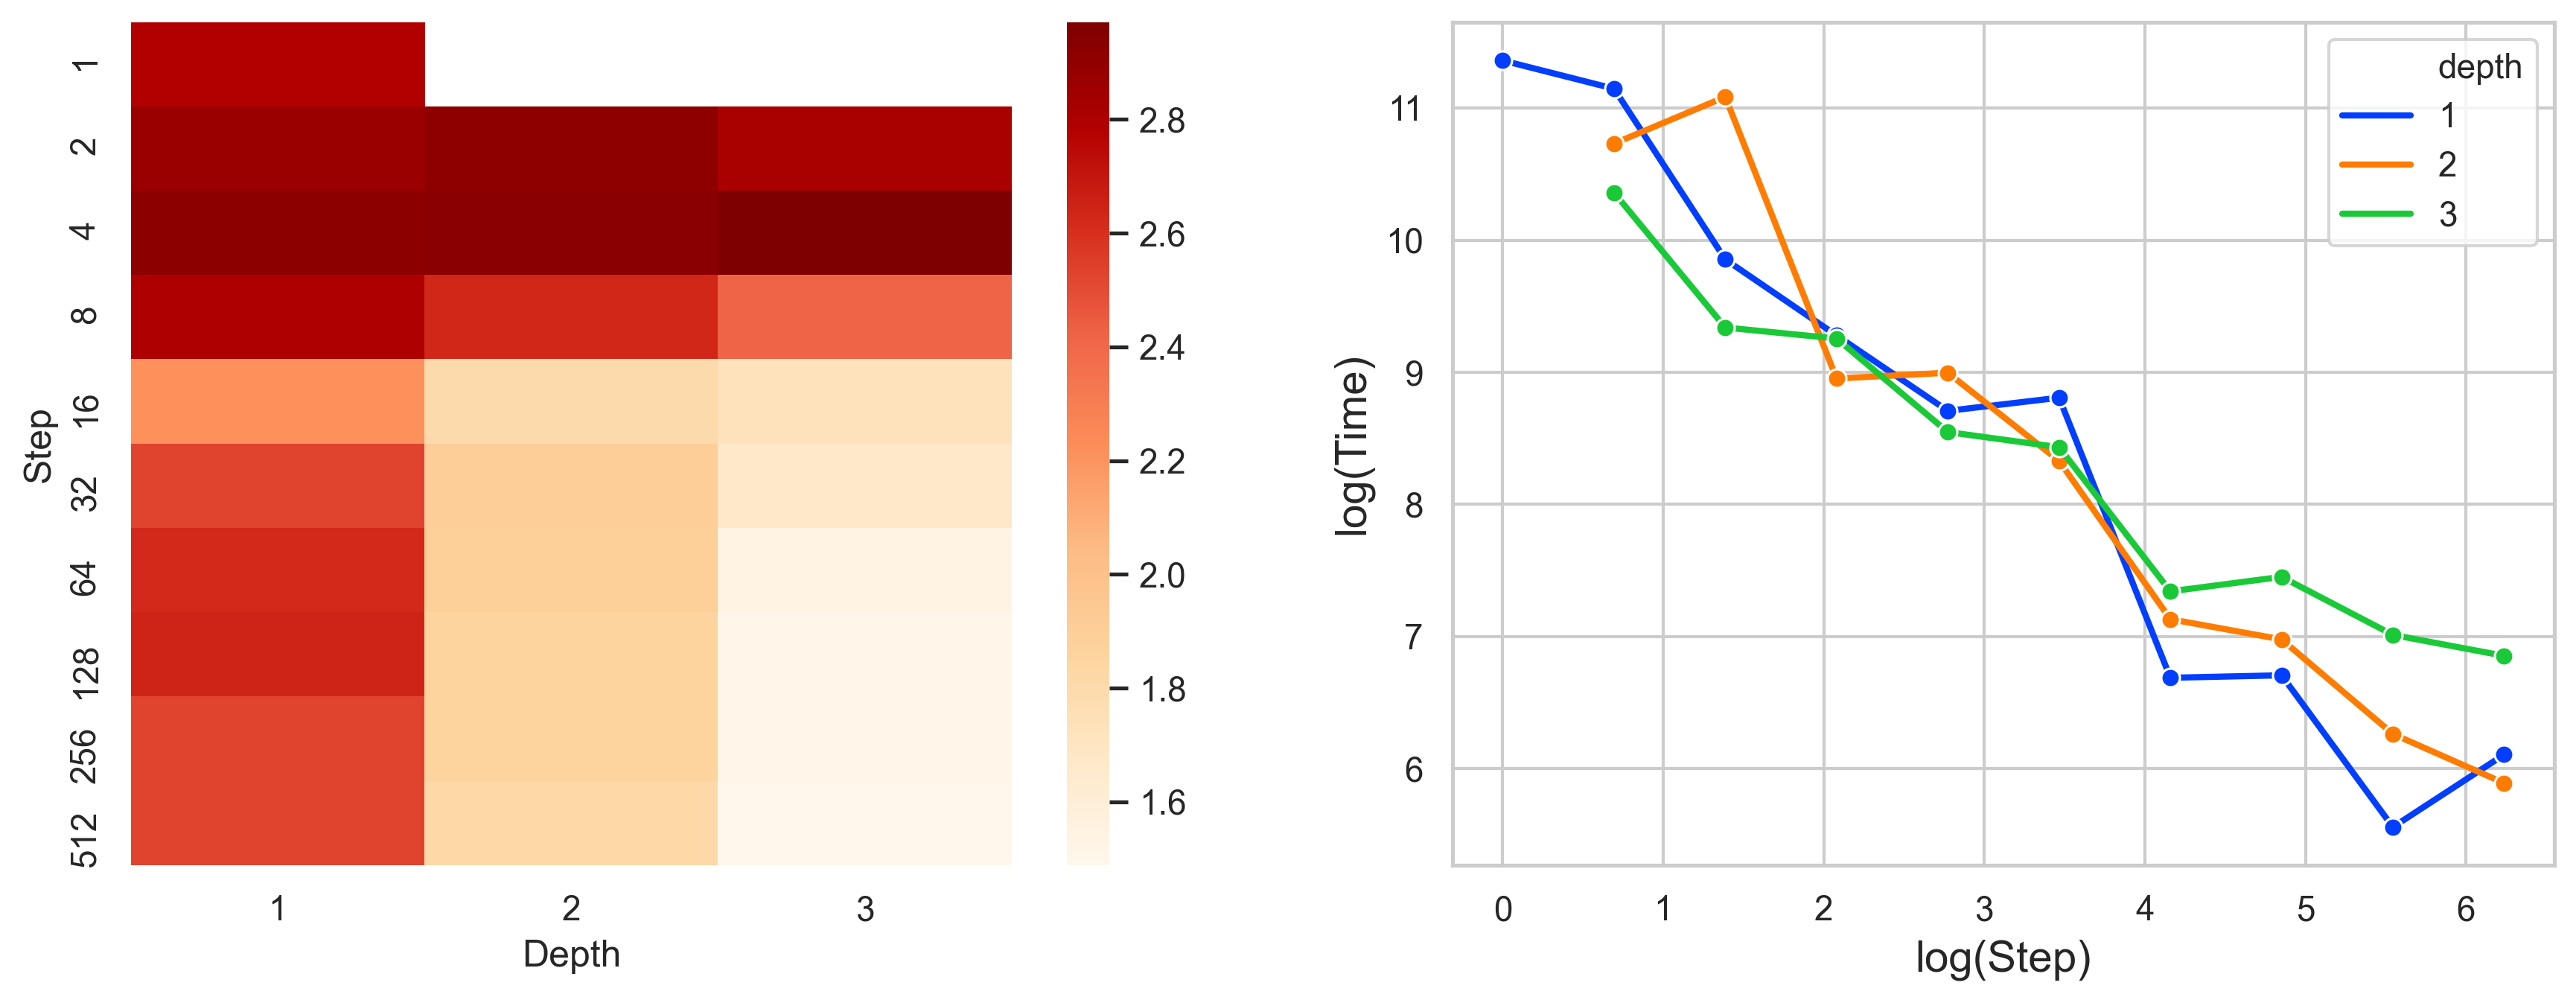
\includegraphics[clip, width=0.95\textwidth]{Images/BIDMCRR.png}%
    }
    
    \subfloat[HR]{
      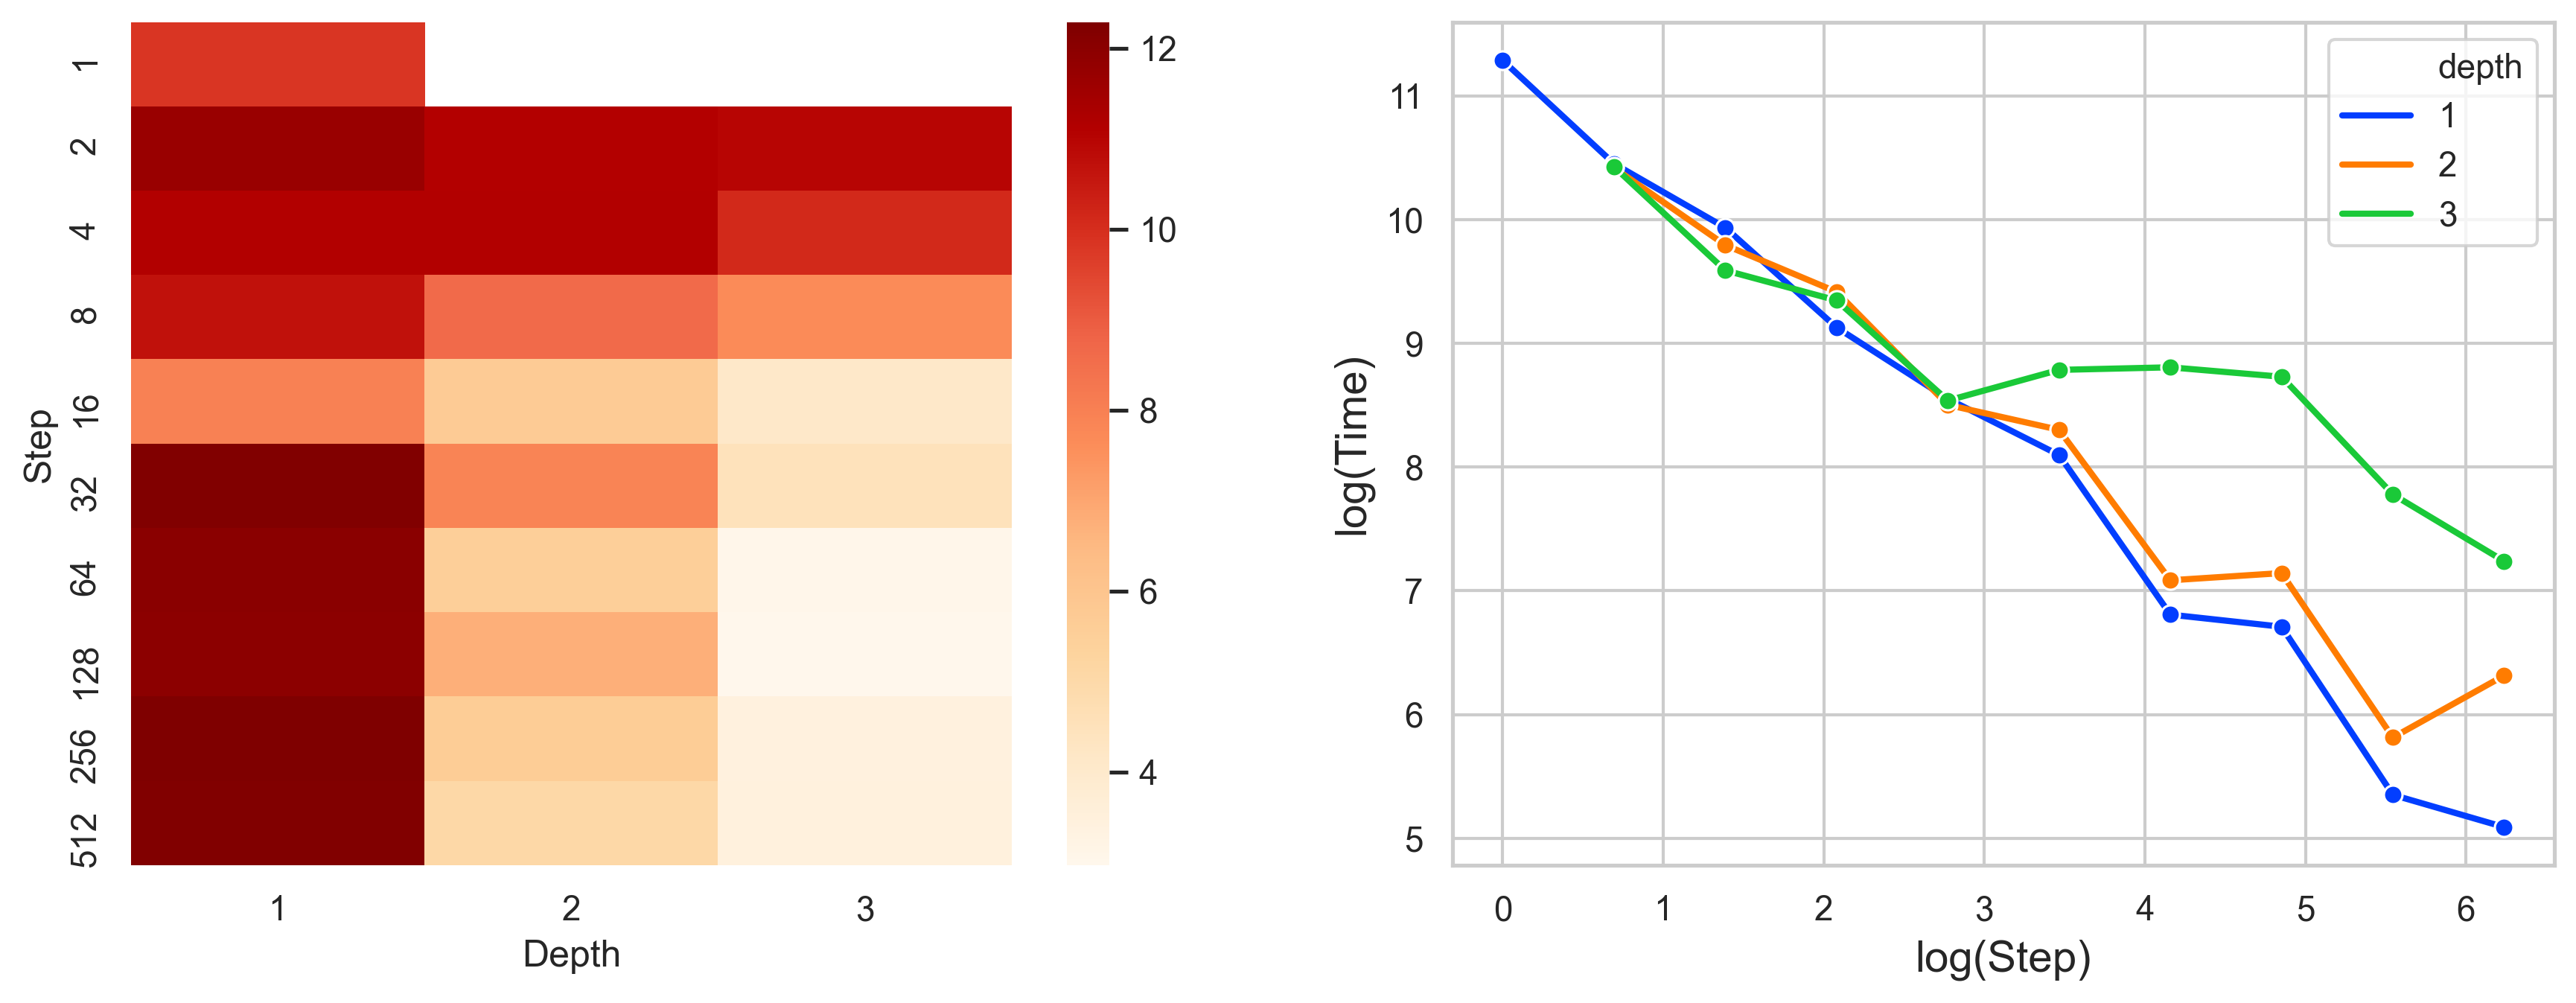
\includegraphics[clip, width=0.95\textwidth]{Images/BIDMCHR.png}%
    }
    
    \subfloat[SpO2]{
      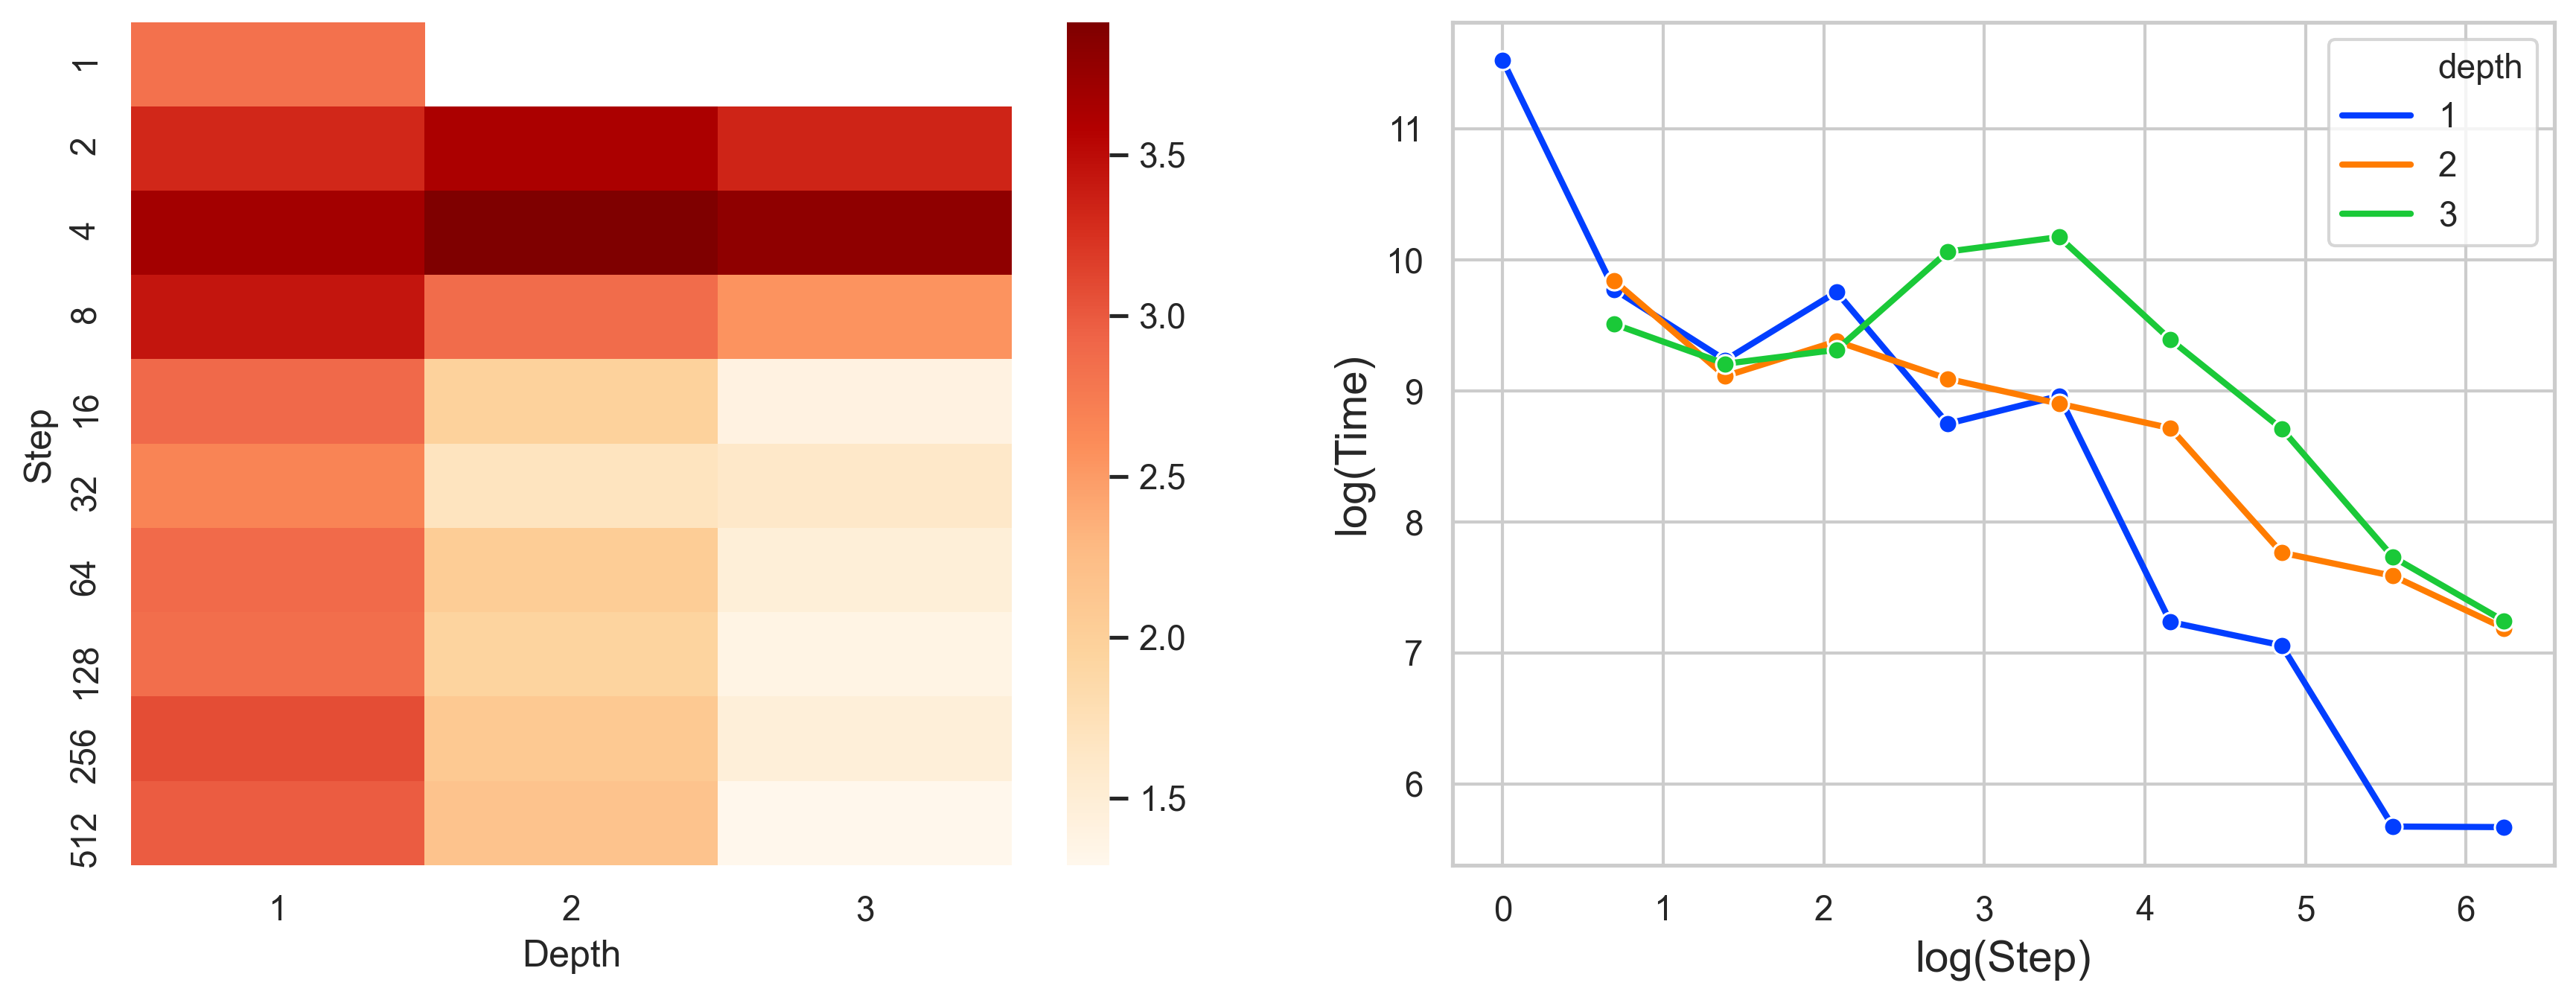
\includegraphics[clip, width=0.95\textwidth]{Images/BIDMCSpO2.png}%
    }

    \caption{Heatmaps of the loss on the test set for the all BIDMC problems and the and a log-log plot of the elapsed time of the algorithm against the step size. Recall that lower is better here unlike for EigenWorms.}
    \label{fig:bidmc_heatmap}
    
\end{figure}
